\documentclass[12pt]{article}
%\usepackage[utf8x]{inputenc}
\usepackage{amsmath}
\usepackage{amssymb}
\usepackage{amsthm}
\usepackage{graphicx}
\usepackage{mathtools}
\usepackage{CJKutf8}

\addtolength{\textwidth}{1.5cm}
\hoffset=-0.7cm
\newcommand{\HH}{\mathcal{H}}
\newcommand{\IP}{\mathbb{P}}
\newcommand{\E}{\mathbb{E}}
\newcommand{\Var}{\mathrm{Var}}
\newcommand{\argmax}{\mathop{\mathrm{arg\,max}}}
\newcommand{\argmin}{\mathop{\mathrm{arg\,min}}}
\newcommand{\eps}{\varepsilon}

\newcommand{\Z}{{\mathbb Z}}
\newcommand{\N}{{\mathbb N}}

\let\phi=\varphi

\newtheorem{theorem}{Theorem}[section]
\newtheorem{corollary}[theorem]{Corollary}
\newtheorem{proposition}[theorem]{Proposition}

\title{The Tangle}
\author{Serguei Popov\thanks{
慣用代稱為 \texttt{mthcl}; 作者聯絡資訊:
\texttt{serguei.popov@iota.org}}
%, for \texttt{Jinn Labs}
}
\date{October 25, 2017. Version 1.4}


\begin{document}
\begin{CJK}{UTF8}{bkai}
 \maketitle
\begin{abstract}  

在本論文中我們分析了 IOTA (一種用於物聯網 [IoT] 行業的加密貨幣) 中所使用的主要技術。
這個新穎的加密貨幣最主要的特點就是 \emph{tangle},以一個有向無環圖 (DAG) 存放交易資訊。
tangle 不僅成功的讓區塊鏈往前邁進一步,其特性更是符合 M2M 小額支付系統的需求。

一個本篇論的關鍵貢獻是馬可夫鏈蒙地卡羅 (Markov Chain Monte Carlo, MCMC) 演算法。
這些演算法會為新的交易選擇要接在哪些既有交易之後。                                        

\end{abstract}

\section{系統介紹與描述}
\label{s_general}

在過去的六年中比特幣的興起和成功證明了區塊鏈技術的價值所在。
然而,這種技術也有許多缺點,阻礙了它成為全球通用的加密貨幣平臺。
在這些缺點中,特別值得提及的就是無法進行小額支付,而小額支付在迅速發展的物聯網行業中的重要性不斷增加。
在現今的系統中,使用者須支付手續費才能產生交易;因此,為了支付極少的金費而須再付好幾倍的手續費並不合理。
且對產生區塊的人而言,手續費就是動機,因此想完全摒除掉並不容易。
另外亦須關注的是現存的加密貨幣都是清楚區分不同角色(如交易發起者,交易驗證者)的異質 (heterogeneous) 系統。
這種明顯區分參與者的設計,容易造成資源搶奪與浪費的現象。
這就需要尋找一些完全不同於比特幣和其他加密貨幣的區塊鏈技術的解決方案。

在本論文中,我們討論了一個創新的方案,但並不能與現今區塊鏈技術相容。
而此方案正以加密貨幣的形式實做,稱之為\emph{IOTA}~\cite{iota},針對物聯網工業所設計。
此篇論文旨在聚焦於 tangle 的一般特性,以及探討當某人試圖捨棄區塊鏈並維護一個分散式帳本時會衍生的問題。
我們並不會討論 iota 具體的實做細節。

在一般情況下,IOTA 按如下方式運行。如前所述,不存在全域的區塊鏈,取而代之的是一個 DAG(有向無環圖),我們稱之為 \emph{Tangle}。
通過節點發出的所有交易構成了這個 Tangle (存所有交易的帳本) 的集合。
這個圖的邊是這樣形成的:當一個新的交易產生,它必須\emph{驗證}之前的兩個\footnote{這是最簡單的方法。
讀者有可能也研讀過相似的系統,規定每筆交易必須驗證 $k$ 筆其他交易,而通常 $k\geq 2$ ,或是採用完全不同的驗證規則。}交易,
這些驗證關係就通過有向的邊來表示,如圖~\ref{f_weights}\footnote{每張圖的時間軸皆為左至右}所示
(在圖中,時間走向皆是從左到右)。
如果從交易~$A$ 到交易~$B$ 之間沒有直接連接的有向邊,而有至少長度為 2 的有向邊路徑存在,我們就說交易~$A$ \emph{間接地驗證}了交易~$B$。
另外,有一個「創世交易」 (genesis trasaction),被所有交易直接或間接驗證,如圖~\ref{f_reverse_weights}。
創世交易的描述如下:在最一開始有一個地址 (address) 擁有全部的 token,接著創世交易會把金錢轉給其他 ``founder'' 的地址。
我們強調所有的 token 皆是創世交易所產生的(不會再產生新的 token),而且不會再有「挖礦」就可以收到金錢獎勵的概念了。\leavevmode\\
術語解釋: \emph{sites}為在 Tangle 圖上的交易;
\emph{節點}(node) 組成整個網路,同時也是交易發起與驗證者。\leavevmode\\
整個架構的宗旨如下:使用者必須驗證其他交易才能發起交易,為整個網路的安全性盡一份力。
我們假設節點檢查認證的交易是否存在衝突。如果節點發現某筆交易與 tangle 的歷史紀錄衝突,便不會直接或者間接的認證具有衝突的交易\footnote{若某節點發起的新交易驗證了衝突交易,
那麼它便有不被其他節點所驗證的風險,而被摒棄。}。
隨著交易被越來越多其他交易直接或者間接的所驗證,這個交易就愈會被系統所接受;
換句話說,要接受一個雙重支付 (double-spending) 交易是極為困難的。
很重要的是我們不會\emph{強制規定}怎麼選擇要驗證的交易;
而是我們認為如果大量的節點依循一些「參考」的規則,
那麼各節點就要分別遵守同類別\footnote{更進一步的論述在~\ref{s_parasite}章節}的規則。這是比較合理的假設,特別是在 IoT,節點是裝載各式韌體的晶片。\leavevmode\\

要發起一個交易,節點需做以下步驟:
\begin{itemize}
  \item 
  根據演算法選擇兩筆交易驗證(這兩筆交易可能會一樣)
  \item 
  檢查這兩筆交易有無衝突,且有皆沒有驗證到衝突的交易
  \item
  要發起一筆合法 (valid) 交易,節點必須解出一道加密的問題,與比特幣相似。
  需要找出一個 nonce 讓其與其他驗證交易的資料的 hash 值為特定格式,如在比特幣的協定中, hash 值得前面需有指定個數個 0
\end{itemize} \leavevmode\\
重要的是, iota 是一個非同步的網路。通常,節點們並不會看到一樣的交易集合。
值得注意的是 tangle 可能存在衝突的交易。
節點間並不需要達成共識,因為合法\footnote{依照協定發起的交易}的交易有權繼續留在帳本中,也就是留在 tangle 中; 
但要是出現衝突的交易,節點便需要決定哪筆交易要被孤立 (orphaned)\footnote{孤立的交易不會再被新進交易間接驗證},也就是這筆交易不會再被新進的交易間接驗證。
決定哪筆交易是要被孤立的主要準則如下: 一個節點進行多次的 tip 選擇演算法\footnote{如上所述,
我們有好的理由可以假設其他節點會遵循一樣的演算法進行 tip 選擇}(cf.\ ~\ref{s_parasite}  節),接著觀察哪筆交易較可能被選到的 tip 間接驗證。
舉例來說: 假設跑了 100 次 tip 選擇演算法,有一筆交易被選到 97 次,我們便說它有 ~$97\%$ 的信心被驗證到。 

我們也一併說明接下來的問題 (cf.\ \cite{red_balloons}): 
促使節點們產生、傳播 (propagate) 交易的動機是什麼? 
每個節點會計算一些數據,其中之一是計算會從鄰居接收多少新的交易。
如果某個特定節點「太懶惰」,便會被它的鄰居捨棄。
因此,即使節點並沒有發起任何的交易,且沒有分享新的交易來驗證自己交易的動力,但他仍然有動機參與。 

在~\ref{s_weight_algo}  節中簡單介紹一些術語後,我們要討論選擇兩筆交易予以接受納入系統的演算法,
用於衡量整體交易的驗證演算法(第~\ref{s_cutsets} 節,尤其是~\ref{s_cum_grow} 節),以及可能會受到的攻擊情況(第~\ref{s_attacks} 節)。 
接著,懼怕數學式的讀者可以直接跳到每一節最後的「結論」。

此外,應該指出的是,有關有向無環圖在加密貨幣領域中的想法已經有一些時日了,
比如文獻 ~\cite{dag_generalized_blockchain, dagcoin, SZ, LSZ, braids}。
尤其需要指出的是,文獻 ~\cite{SZ} 中提出是被稱為 GHOST 的協議,修改了比特幣協議,把主要帳本的結構從區塊鏈改為一棵樹(tree); 
這樣的作法顯示,可以降低驗證時間並提高整體網路的安全性。
在文獻~\cite{LSZ} 中,作者們提出了基於 DAG 的加密貨幣模型; 
有別於我們模型的是,組成 DAG 的是區塊 (block),而非獨立的交易。
且礦工會競爭手續費,新的金錢也會被創造。
再來,文獻~\cite{dagcoin} 中提出了一種類似於我們的解決方案,雖然他並沒有討論任何驗證 tip 的方法。
在這篇論文發布後,也有其他人也研究以 DAG 為基礎的分散式帳本,如~\cite{SZ_SPECTRE}。
我們也提及了另一種~\cite{bitcoinj,lightning} 針對基於 P2P 的比特幣小額支付的解決方案。

\section{權重及相關概念}
\label{s_weight_algo}
本節我們定義一個交易的自身權重及其相關概念。交易的權重與發送這筆交易的節點所投入的工作量成正比;
在目前 iota 的實作中,權重可以假定為 $3^n$ 的一些數值,其中 $n$ 屬於有限區間內的正整數\footnote{這個區間應為有限的 --- 
參照第~\ref{s_attacks} 節中的「大權重攻擊」}。
事實上,這與權重是如何增加的並不相干; 重要的是,每一筆交易都有一個正整數的權重。
總之,權重愈高該筆交易在 tangle 中也就愈「重要」。
為了避免各式攻擊,我們假設沒有任何角色 (entity) 可以在短時間內產生大量的「可接受」權重的交易。
 
我們所需要的一個重要概念就是一個交易的\emph{累積權重}:
它被定義為這個交易的自身權重與其他直接以及間接驗證這個交易的所有交易的自身權重之和。
累積權重的計算方法如圖~\ref{f_weights} 所示。其中方框代表交易,方框右下角較小的數字表示這個交易的自身權重,
而字體加粗的數字是這筆交易的累積權重。例如,交易~$F$ 經交易 $A,B,C,E$  直接或者間接被驗證。
交易~$F$ 的累積權重就是交易 $A,B,C,E$ 的各自自身權重之和,即 $9=3+1+3+1+1$。

在圖~\ref{f_weights} 中沒有被驗證的交易(即 “tips”)只有交易~$A$ 和交易~$C$。
若一個新的交易~$X$ 進入系統並且驗證交易~$A$ 和~$C$,那麼交易~$X$ 就是系統中唯一的 tip 了,
同時系統中其他所有的交易的權重增加 3(即交易~$X$ 的自身權重)。
為了討論驗證演算法,我們需要引入一些其他的變數。

\begin{figure}
 \centering 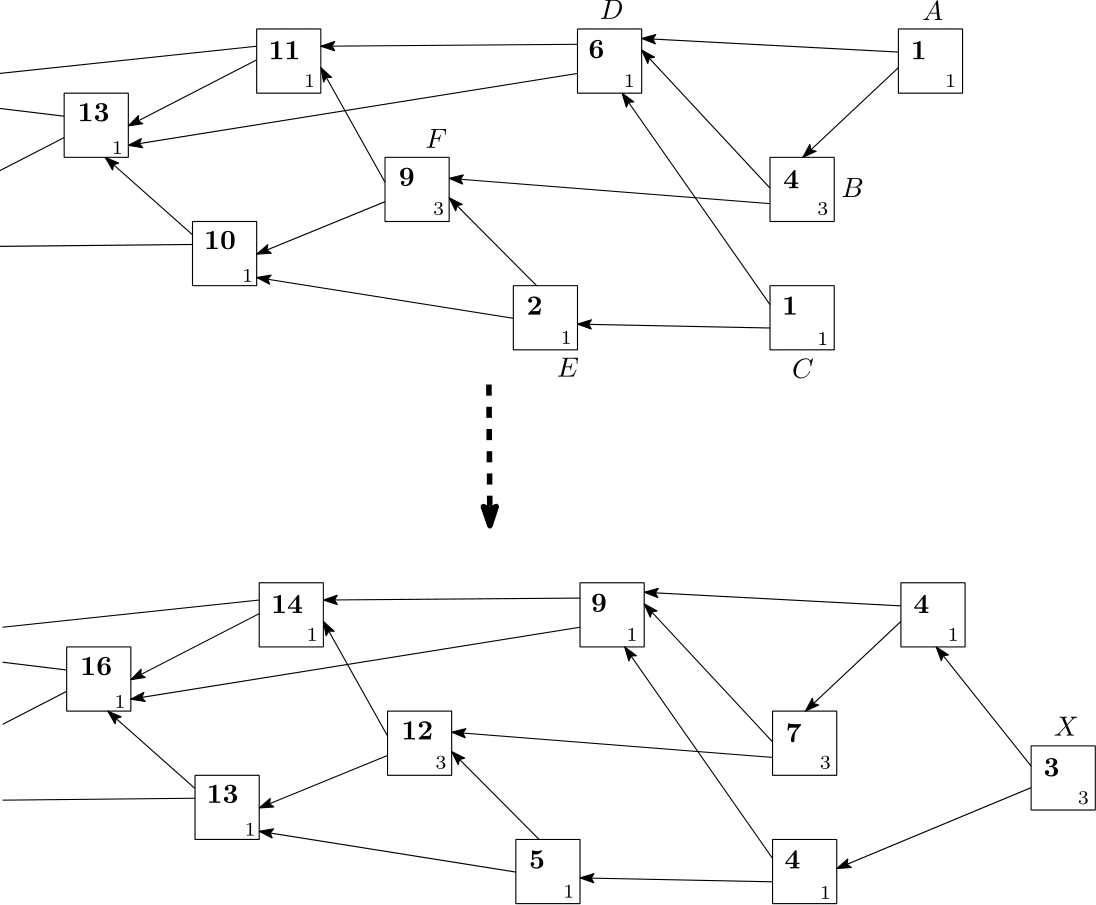
\includegraphics[width=0.64\textwidth]{weights} 
\caption{新發起交易進入系統後的權重改變圖。每個方框代表交易,
方框右下角較小的數字表示這個交易的自身權重,
而粗體數字是每筆交易的累積權重。}
\label{f_weights}
\end{figure}

在討論驗證演算法前,我們須再介紹兩個名詞:
首先,對於 tangle 中的一筆交易,它的:
\begin{itemize}
 \item \emph{高度}(height): 定義為自創世交易 (genesis) 至當前這個交易的所有路徑中最長的長度
 \item \emph{深度}(depth): 定義為自這個交易到某個 tip 的最長路徑;
\end{itemize}

例如,在圖~\ref{f_reverse_weights} 中,交易 $G$ 的高度為 1,深度為 4 (因為反向路徑 $F,D,B,A$);
而交易~$D$ 的高度為~$3$,深度為~$2$。
接下來,我們引入\emph{積分} (score) 的概念。
一筆交易的積分定義為它的自身權重與所有它驗證的那些交易的自身權重之和。

\begin{figure}
 \centering 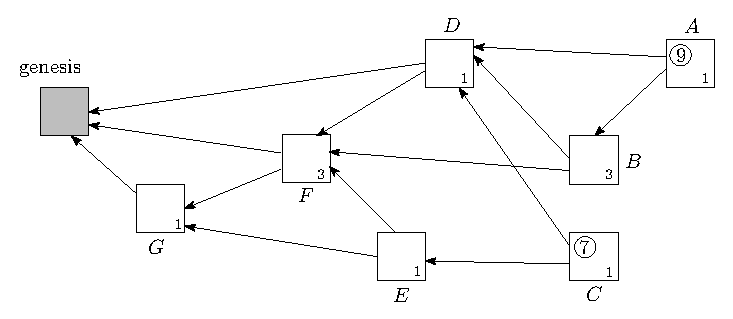
\includegraphics[width=0.64\textwidth]{reverse_weights} 
\caption{
每筆交易的自身權重,以及交易~$A$ 和~$C$ 的積分}
\label{f_reverse_weights}
\end{figure}

在圖~\ref{f_reverse_weights} 中,僅有的 tips 有交易~$A$ 和~$C$。
交易~$A$ 直接或者間接地驗證了交易 $B,D,F,G$,因此交易~$A$ 的積分為 $1+3+1+3+1 = 9$。
同樣地,交易~$C$ 的積分為 $1+1+1+3+1 = 7$。

想要了解本論文的證明過程,你可以假設所有交易的權重都為 1。
因此,\emph{從現在開始,我們會依循這個假設}。
在這個假設底下,交易~$X$ 的累積權重就是~$1$ 加上所有直接或間接驗證~$X$ 的交易個數,
而積分則為~$1$ 加上被~$X$ 直接或間接驗證的交易個數。

接著注意到,所有代數中最重要的就是累積權重(就目前而言!),而高度、深度以及分數待會也會列入討論。


\section{系統的穩定性和截斷集合}
\label{s_cutsets}

記 $L(t)$ 為 $t$ 時刻系統中 tips 的總數。
當然,大家預期隨機變數 $L(t)$ 保持\emph{穩定}\footnote{在整個發展過程與時間皆同步的假設下},
更精確地來說,我們期望是\emph{正遞迴} (positive recurrent) 的; 
正式的定義可以參照第~4.4 節以及~\cite{Ross_m} 的~6.5 節處; 
正遞迴指的是當 $t\to\infty$,$\mathbb{P}\big[L(t)=k\big]$ 的極限應存在且為正值 $\forall k\geq 1$ )。
直觀上, $L(t)$ 應當圍繞一個恆定的常數波動,而不是趨於無限大。
如果 $L(t)$ 趨近於無限大,這樣的話系統中會存在大量未經驗證的交易。

為了分析 $L(t)$ 的穩定性,我們需要一些前提假設。
其中一個就是,當有一個獨立的節點產生了一個大權重的交易,
因此新進交易的整個過程可以以帕松分佈為模型(cf.\ e.g.\ ~\cite{Ross_m} 的~5.3 節)。
假設 $\lambda$ 為帕松過程 (Poisson process) 的交易輸入流的速率;為簡單起見,我們假定交易輸入流的速率隨著時間仍保持恆定。
假設所有的設備都具有相近的計算能力,一台設備要發送一筆交易所需要計算的平均時間為 $h$。
我們\emph{假定}所有節點都符合以下模式:
 
即在要發送一筆交易的時候,節點從 tips 中隨機選擇兩個並驗證它們。
須注意到的是,對「誠實的節點」而言,採用此方法並\emph{不是}一個好主意。
有幾個缺點,它並不能有效的抵制「懶惰的節點」和惡意的節點(參照第~\ref{s_parasite} 節)。
但我們仍把這個方法納入討論,因為其較容易分析,而且讀者也接著會一窺較複雜的 tip 選擇演算法。

接下來我們做進一步的簡化,當一個節點發起交易時,它並非是 tangle 真正的樣貌,而是~$h$ 個時間單位以前的狀態。
這代表通常一個交易在時間~$t$ 接上 tangle 後,要到時間~$t+h$ 才會在 tangle 上看見。
我們也假定 tips 的總數保持在幾乎靜值,數字大概落在 $L_0>0$ 上下,在接下來我們會計算由 $\lambda$ 與 $h$ 推導的 $L_0$ 函數。

我們發現,在一個給定的時間 $t$,我們有約 $\lambda h$ 的「隱藏的 tip」(這些 tips 是在時段 $[t-h,t)$ 接在 tangle 上,
所以它們尚未能在 tangle 上看到);接著我們假設有 $r$ 個「顯現的 tips」(在~$t-h$ 之前接上 tangle 的 tips),
所以得出 $L_0=r+\lambda h$。由於 tips 的總數是穩定的,我們或許可假設有 $\lambda h$ 個交易在~$t-h$ 的時候為 tips 而在時間 t 時已不是了。
現在考慮一個全新的交易被引進的情況;則這個交易會驗證到 tips 的機率為 $r/(r+\lambda h)$
(因為這裡有 r 個 tips,而這裡也有 $\lambda h$ 個不是 tips 但節點誤以為是),所以選擇到 tips 的期望值是 $2r/(r+\lambda h)$。
我們可以發現一個重要的現象,在穩定的狀態中,選擇到 tips 的期望值為 $1$,因為就平均而言,一個新進的交易並不會改變 tips 的總數。
解 $2r/(r+\lambda h)$,可以得到 $r=\lambda h$,以及
 
\begin{equation}
\label{L0_def} 
L_0 = 2\lambda h.
\end{equation}

我們在這裡註記,如果今天規則改成一個交易會去驗證~$k$ 個交易,而非兩個,則我們有類似的計算:
\begin{equation}
\label{L0k_def} 
 L_0^{(k)} = \frac{k\lambda h}{k-1}.
\end{equation}
理所當然的,$L^{(k)}_0$ 會趨近於 $\lambda h$ 當 $t$ 趨近無限大(基本上,剩下的 tips 會是那些網路上尚未可見到的)

我們回去考慮會有兩個交易會被驗證的情況,一個交易第一次被驗證時間預計約為 $h+L_0/(2\lambda)=2h$。
因為根據我們的假設,在第一個~$h$ 個單位時間之前,交易是不會被驗證的。
接下來驗證此交易的帕松過程的速率為 $(2\lambda)/L_0$ (可參考~\cite{Ross_m} 的~5.3,
說明了當我們以不同類別獨立分類每個帕松過程,那麼各個類別的帕松過程是相互獨立的)。

同時,注意到\footnote{至少在交易節點\emph{試圖}驗證 tips 的情況下} 對任意固定 $t$ 時刻, 
在某一個階段 $s\in\big[t,t+h(L_0,N)\big]$ 內那些 tips 構成了一個\emph{截斷集合}(cutset),
在時間 $t'> t$ 時發起的交易到創世交易的任何路徑都必須通過這個集合。
很重要的是,在某些情況下這個會截斷集合變得非常小。
我們也許可以使用這個較小的截斷集合作為檢查點,作為 DAG 可能的剪枝或者其他用途。 

上述「純隨機」策略實際上並不太好,因為這種策略不會鼓勵節點驗證交易:
比如「懶惰」的用戶也許總是去驗證較早的幾筆固定交易,因此就沒有貢獻到較新交易的驗證,而這種行為也不會受到懲罰。\footnote{
提醒讀者,我們並非嘗試 \emph{強迫推行} 任何一種 tips 選擇方式。攻擊者能以任何它覺得便利的方式選擇 tips。)}
惡意的節點也可以產生大量交易驗證幾組固定交易達到人工製造大量 tips,讓未來的新交易能有極高機率選擇這些 tips,
而有效的捨棄「誠實」節點的 tips。
為了避免這個行為,我們得採用另一種方法,讓新進交易偏向選擇「好」的 tips。
在~\ref{s_parasite} 節有一個此種策略的例子。\footnote{作者認為,以 tangle 為基礎的加密貨幣中最重要的元素是 tip 驗證的方法,
因為攻擊的途徑就隱含於其中。此外,既然通常不會強制以什麼方法驗證 tip,則必定存在一個讓節點自願依循某個常見方法的理由。
一個可能的原因是節點知道有相當多的其他節點都遵照同一個 tip 的驗證方法。}

在討論交易第一次被驗證所需時間的期望值前,我們分兩個區間進行分析,(圖~\ref{f_regimes})。

\begin{itemize}
 \item 低負載區: tips 的數量很少,常常只有 1 個。
 當交易流足夠慢時會發生,不太可能發生不同的交易驗證同一個 tip 的情況。
 而且若網路延遲很短且設備運算的速度很快,也不大可能會有大量 tips 出現的情況。
 即使是在交易流的很快的情況下也是如此。此外,我們也應假設不會有攻擊者產生大量的交易以膨脹 tips 數量。
 \item 高負載區: tips 的數量很多。當交易流很大且計算力與網路的延遲很長時便可能會讓多筆不同交易驗證到同一個 tip。
\end{itemize}
\begin{figure}
 \centering 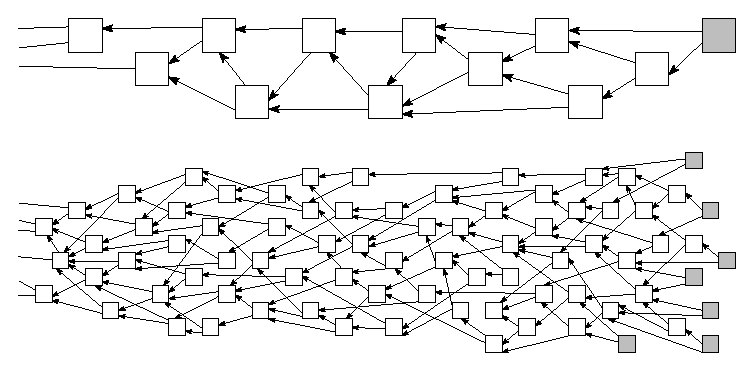
\includegraphics[width=0.64\textwidth]{regimes} 
\caption{新進交易的低負載 (上方) 與高負載 (下方)。白框代表合法的交易,灰框則表示 tips。}
\label{f_regimes}
\end{figure}

這樣的分法是比較不正式,且在這兩個區間中並沒有明顯的分界線。然而,我們認為討論這兩種極端是有啟發的。

在低負載區域,這種情況就相對簡單:在 $\lambda^{-1}$ 的時間尺度上會有第一次驗證, 
因為第一批中的一個新進交易將會驗證我們的這些 tips。

現在我們來考慮高負載區域的情況,當 $L_0$ 很大的時候。
如上面所提到的,我們可以假設驗證其他 tips 的帕松事件是相互獨立且其機率近似 $2\lambda/L_0$。
因此,我們預期一筆交易被第一次驗證的時間約為 $L_0/(2\lambda)\approx1.45h$~\eqref{L0_def}。

值得一提的是,更好的驗證策略\footnote{在未來 iota 的實做中,會偏袒「好」的 tips},花費大量時間等待交易被驗證並不是個好主意,
這是因為「好」的 tips 會不斷的出現且也常被選擇驗證。
甚至當交易在等待被驗證的時間大於 $L_0/(2\lambda)$ 時,一個好的辦法就是另外發起一個空交易\footnote{空交易就是筆沒有 token 的轉帳,
但仍須驗證兩筆其他交易。注意到,產生空交易還是會貢獻整個網路的安全性。}。換言之,
節點能發起一個新的空白交易選擇其他「好」的 tips 和它之前的交易驗證,這便會讓這個空白交易會有很大的機會被驗證。

原本基於高度 (heights) 和積分 (scores) 的驗證策略可能會受到特定類型的攻擊,見~\ref{s_parasite} 節分析。
我們將在那一節中討論更加詳細的策略\footnote{事實上,作者認為,以 tangle 為基礎的加密貨幣中最重要的元素是 tip 驗證的方法,
因為很多的攻擊途徑就隱含於其中。此外,既然通常不會\emph{強制}以什麼方法驗證 tip,則必定存在一個讓節點自願依循某個常見方法的理由。
一個可能的原因是節點知道有相當多的其他節點都遵照同一個 tip 的驗證方法。}來防止這樣的攻擊。
同時,這種隨機驗證兩筆交易的 tip 選擇策略最簡單,但仍然是值得考慮的。這個策略的分析最簡單,
從而可能會給出 tangle 行為方面的一些定性和定量方面的理解。

\paragraph{結論:}
\begin{enumerate}
 \item 我們區分了兩個區間,低負載和高負載區間,如圖~\ref{f_regimes} 所示。
 \item 在低負載區,tips 不多,一個 tip 在 $\Theta(\lambda^{-1})$ 時間尺度內得到第一次驗證,
 其中 $\lambda$ 是進入系統內的交易流速度。
 \item 在高負載區,tips 的典型數量取決於新進交易使用的驗證策略
 \item 若一筆交易採用「隨機驗證兩個 tips」策略,tips 的典型數量由公式~\eqref{L0_def} 決定。
 可以看到這種策略在 tips 的典型數量上是理想的,但是在實際中不會選用這種策略,因為此策略不會鼓勵新的交易去驗證 tips。
 \item 我們需要更多精巧的方法以抵擋攻擊與整體網路的問題,這類方法將在~\ref{s_parasite} 節中進行討論。
 \item 在高負載區,一個 tip 獲得驗證所需要的時間尺度為 $\Theta(h)$,其中 $h$ 是一個節點的平均計算/廣播時間。
 但是,如果在上述時間間隔內沒有獲得第一個驗證,那麼額外發送一筆空白交易提高驗證速度,對於交易產生者或接收者便是一個好方法。
\end{enumerate}




\subsection{累積權重的增長有多快?}
\label{s_cum_grow}

假設網路是在低負載區,在交易被驗證幾次後,它的累積權重將以 $\lambda$ 的速度增加,因為所有新的交易都將間接指向這筆交易\footnote{
回顧之前我們假設所有交易的自身權重皆為~$1$,因此其累積權重就會是直接或間接指向這此交易的交易數目加~$1$。}。

而若在高負載區,具有較大的累積權重的舊交易,其累積權重同樣會以 $\lambda$ 的速度增加,因為基本上新進的交易都會間接的指向它。
此外,當交易剛進入 tangle 時需要等待一定的時間被驗證,而在這段時間內,其累積權重會以較為無規的形式增長。
為了弄明白一個交易在得到幾個驗證之後其累積權重的變化行為,
我們記 $H(t)$ 為 $t$ 時刻該交易的累積權重期望值,(為簡單起見,我們自發起交易開始計時,也就是在發起交易的 $h$ 時間單位後)
並用 $K(t)$ 表示在 $t$ 時刻驗證我們的這筆交易的 tips 數量的期望值。在此,我們簡記為 $h:=h(L_0,N)$。
同時,我們做一個簡化假設,認為 tips 的總數大體保持恒定不變,其值約為 $L_0$。本節我們採用「隨機驗證兩個 tips」的策略;
可預期其結果大致上與其他合理的策略的結果相同。

在 $t$ 時刻進入網路中的一筆交易通常是基於 $t-h$ 時刻時網路的狀態,來選擇兩筆交易進行驗證,因為節點在真正發起交易前必須進行一些運算和驗證。
不難得到(假設,$K(\cdot)$ 是 \emph{真實的} tips 個數, 而非期望值)一筆交易至少驗證一個「我們的」 tip 的機率是 
$1-\big(1-\dfrac{K(t-h)}{L_0}\big)^2=\dfrac{K(t-h)}{L_0}\big(2-\dfrac{K(t-h)}{L_0}\big)$\footnote{
等號左手邊的 1 減掉 2 個不是我們的 tips 被驗證的機率}。
因此我們可以寫下如下的微分方程 (類似於文獻~\cite{Ross_m}中的例子 6.4):

我們可以得知 $\delta>0$
\[
 H(t+\delta) = H(t) 
+ \lambda \delta\frac{K(t-h)}{L_0}\Big(2-\frac{K(t-h)}{L_0}\Big)
 + o(\delta),
\]
我們可以化簡式子為︰
\begin{equation}
\label{diff_H}
 \frac{d H(t)}{dt} = \lambda \frac{K(t-h)}{L_0}\Big(2-\frac{K(t-h)}{L_0}\Big).
\end{equation}
為了能夠使用方程式~\eqref{diff_H},我們首先需要計算 $K(t)$。計算 $K(t)$ 是很困難的,
因為在 $t-h$ 時刻的一個 tip 也許在 $t$ 時刻已經不是一個 tip。並且,在新進入的交易驗證了這樣一個 tip 的情況下,
那麼驗證原來交易的 tips 總量就會增加 1 個。現在,
可以觀察到一個關鍵是在 $t-h$ 時刻的一個 tip 在 $t$ 時刻仍然保持為 tip 的機率為 $1/2$。
(欲驗證此,回顧在第~\ref{s_cutsets} 節的討論: 典型的 tip 數目為 $2\lambda h$,而在~$h$ 時間後,$\lambda h$ 個新的 tips 會替換舊的一半。)
因此,在 $t$ 時刻,有 $K(t-h)$ 的一半的「以前」的 tips 仍然保持為 tips,而另一半已經至少被一筆交易所驗證。

讓我們用~$A$ 表示 $K(t-h)/2$ 個在 $t-h$ 到 $t$ 時刻仍然保持為 tips 的這些交易的集合,
而用~$B$ 表示另外 $K(t-h)/2$ 個在 $t$ 時刻已經被驗證過的 tips 的集合。
假定新進入的交易至少驗證了集合~$B$ 中一筆交易而沒有驗證集合~$A$ 中任何交易的機率為 $p_1$;
接著假設同時驗證了兩筆集合~$A$ 中的交易的機率為 $p_2$ 。換言之, $p_1$ 和 $p_2$ 分別對應於在新交易到達時,
目前「我們」的 tips 增加或者減少 1 的機率。因此,得到一些基本關係式:

\begin{align*}
 p_1 &= \Big(\frac{K(t-h)}{2 L_0}\Big)^2 + 2\times
\frac{K(t-h)}{2 L_0}\Big(1-\frac{K(t-h)}{L_0}\Big),  \\
 p_2 &= \Big(\frac{K(t-h)}{2 L_0}\Big)^2.
\end{align*}
為了得到第一個敘述,觀察到 $p_1$ 等於都驗證~$B$ 集合的機率與第一個驗證~$B$ 集合且第二個不是 $A\cup B$ 集合的機率之和,類似方程式~\eqref{diff_H},
$K(t)$ 的微分方程:
\begin{equation}
\label{diff_K}
 \frac{d K(t)}{dt} = (p_1-p_2)\lambda = \lambda
 \frac{K(t-h)}{ L_0}\Big(1-\frac{K(t-h)}{L_0}\Big).
\end{equation}
很難準確地求解方程~\eqref{diff_K},因此我們進一步簡化假設。首先,我們可以看到,對於任意固定 $\epsilon >0$ ,
在當 $K(t)$ 達到 $\epsilon L_0$ 水準之後,它將會迅速增長到 $(1-\epsilon)L_0$ 。
現在,當 $K(t)$ 相對於 $L_0$ 非常小的時候,我們可以捨棄掉方程~\eqref{diff_K}\footnote{得到一個接近~$1$ 的常數,因此等號右邊會等於
$\lambda\frac{K(t-h)}{ L_0}$。} 右邊最後一項。
藉由 $\dfrac{\lambda h}{L_0}=\dfrac{1}{2}$ ,我們可以得到方程~\eqref{diff_K} 的簡化版:
\begin{equation}
\label{diff_K_simpl}
 \frac{d K(t)}{dt} \approx \frac{1}{2h}K(t-h),
\end{equation}
其中邊界條件為 $K(0)=1$。我們打算尋找 $K(t)=\exp(c\dfrac{t}{h})$ 形式的解;帶入~\eqref{diff_K_simpl} 之後,我們得到:
\[
 \frac{c}{h}\exp\Big(c\frac{t}{h}\Big) 
   \approx \frac{1}{2h}\exp\Big(c\frac{t}{h}-c\Big),
\]
因此 
\begin{equation}
\label{eq_K_simpl}
K(t)=\exp\Big(W\big({\textstyle\frac{1}{2}}\big)\frac{t}{h}\Big)
    \approx \exp\Big(0.352\frac{t}{h}\Big)
\end{equation}
這是一個近似解,這裡的~$W(\cdot)$ 是所謂的 Lambert $W$-function。\footnote{也稱為 omega function 或 product logarithm; 
在~$x\in [0,+\infty)$,由 $x=W(x)\exp(W(x))$ 這個關係式的特性。}
同時對式~\eqref{eq_K_simpl} 左右兩邊取對數,我們可以得到~$K(t)$ 達到 $\epsilon L_0$ 所需要的時間大約為:
\begin{equation}
 \label{eq_t0}
 t_0 \approx \frac{h}{W\big({\textstyle\frac{1}{2}}\big)} 
\times \big(\ln L_0 - \ln \eps^{-1}\big)
\lesssim 2.84 \cdot h  \ln L_0.
\end{equation}
再回到方程~\eqref{diff_H},並且如前面一樣捨棄掉右邊最後一項),我們可以得到在 「調整階段」
(例如,在 $t\leq t_0$ 的時候, $t_0$ 為~\eqref{eq_t0} 式的結果) 具有如下方程:
\begin{align*}
 \frac{d H(t)}{dt} &\approx \frac{2\lambda}
{L_0}K(t-h)
  \\
&\approx \frac{1}{h\exp\big(W(\frac{1}{2})\big)}
\exp\Big(W\big({\textstyle\frac{1}{2}}\big)\frac{t}{h}\Big)
\\
&= \frac{2W\big({\textstyle\frac{1}{2}}\big)}{h}
\exp\Big(W\big({\textstyle\frac{1}{2}}\big)\frac{t}{h}\Big)
\end{align*}
因此,
\begin{equation}
\label{eq_H}
 H(t)\approx 
2\exp\Big(W\big({\textstyle\frac{1}{2}}\big)\frac{t}{h}\Big)
\approx 2\exp\Big(0.352\frac{t}{h}\Big).
\end{equation}

在此提醒讀者,在調整階段之後,累積權重 $H(t)$ 會隨著速度 $\lambda$ 線性增長。
我們需要強調的是在~\eqref{eq_H} 式中的「指數增長」並不意味著在調整階段累積權重增長「十分的迅速」,圖~\ref{f_adapt_period} 中描述了其行為。
\begin{figure}
 \centering 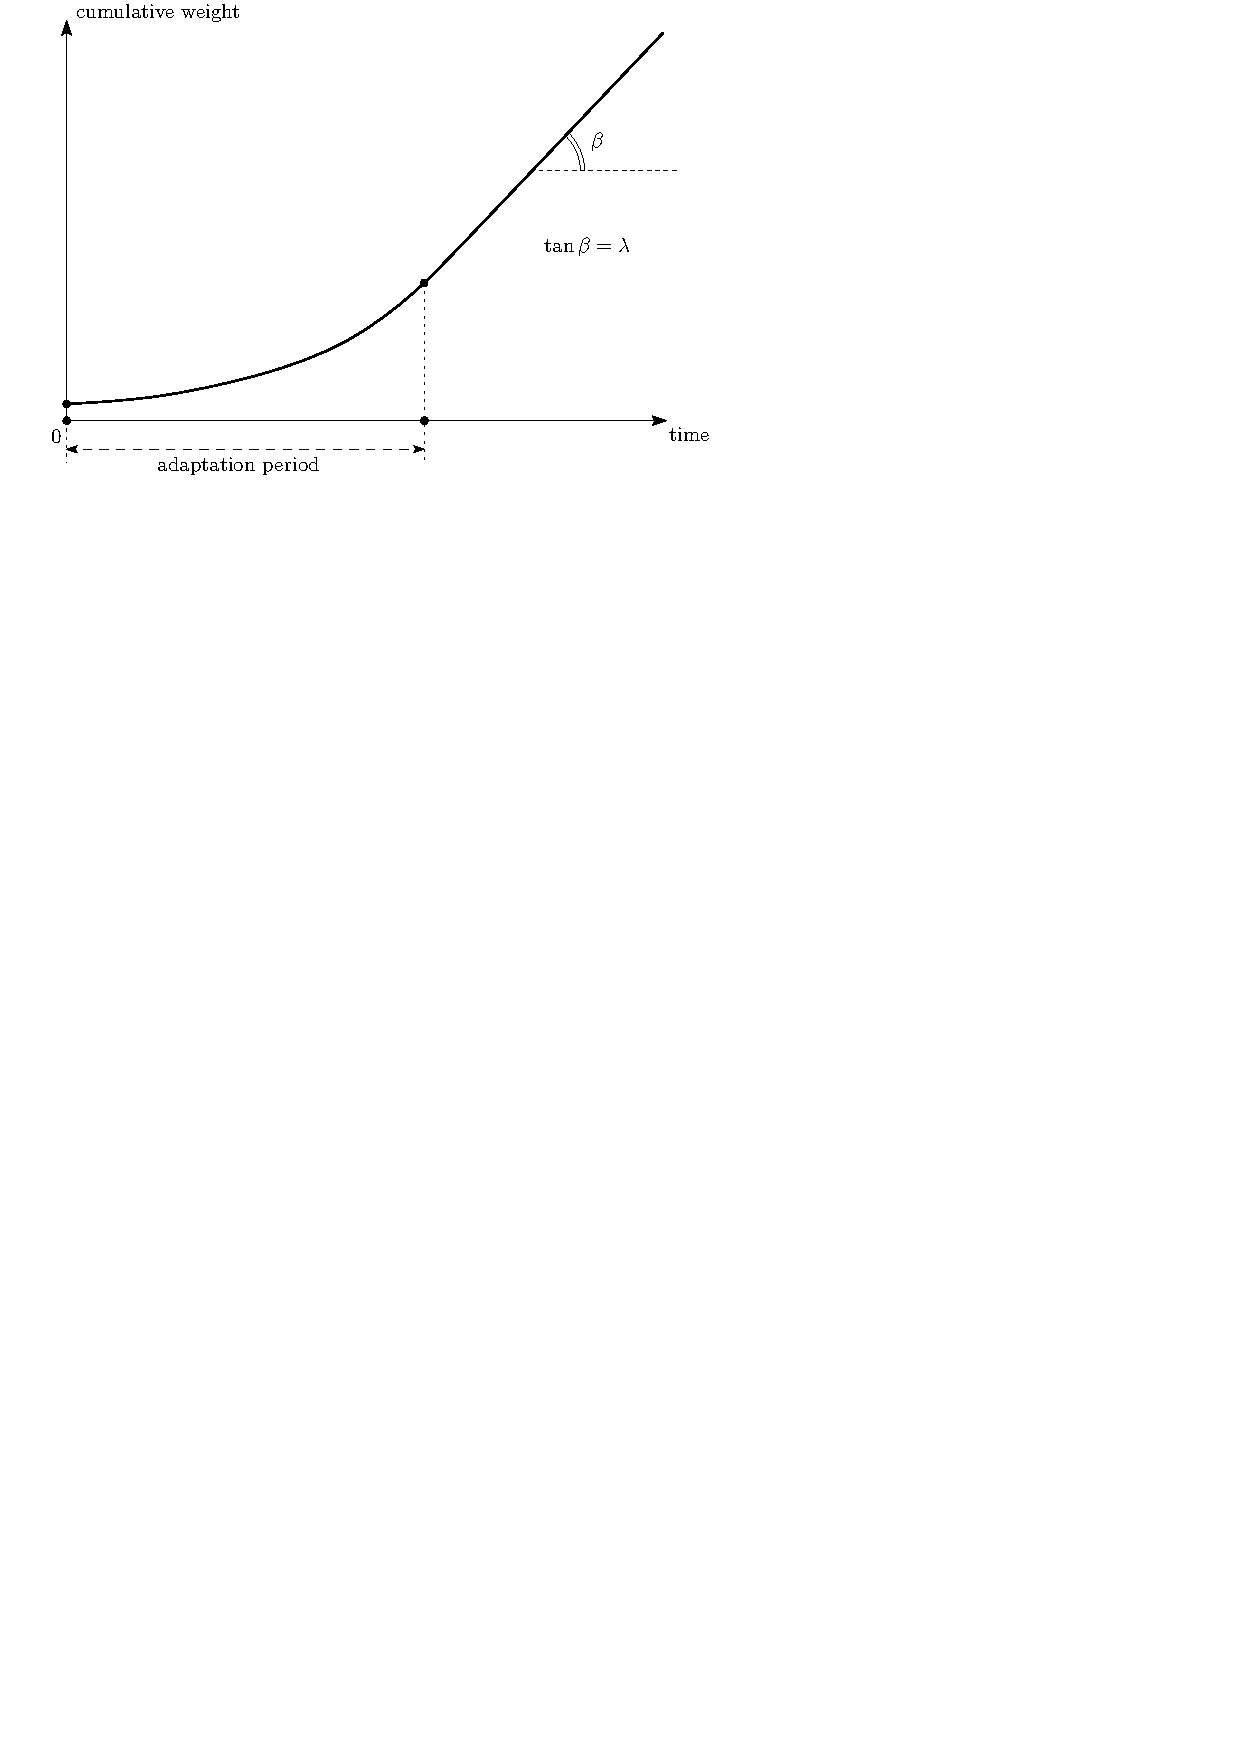
\includegraphics[width=0.64\textwidth]{adapt_period_1} 
\caption{累積權重 v.s. 高負載區的時間}
\label{f_adapt_period}
\end{figure}

\goodbreak

\paragraph{結論}
\begin{enumerate}
 \item 在低負載區中,一筆交易被驗證過多次以後,其累積權重會以~$\lambda w$ 的速度增加,其中~$w$ 是一般交易的平均數。
 \item 在高負載區中,會有兩種不同的狀態。其一,根據方程~\eqref{eq_H},一個交易在\emph{調整階段} 的累積權重~$H(t)$ 會以飛快的速度增加。
 在調整階段結束後,累積權重的增長速度為~$\lambda w$ (圖~\ref{f_adapt_period})。事實上,對於\emph{任何}合理的策略,
 累積權重都會以這個速度增加。因為所有新進的交易都會間接的驗證此交易。
 \item 您可以視一個交易被現在的 tips 間接驗證的這段時間為適應階段。
而其標準的適應階段長度由~\eqref{eq_t0} 得出.
\end{enumerate}


\section{可能的攻擊情況}
\label{s_attacks}
讓我們在討論一個攻擊方案,當攻擊者試圖「趕上」整個網路:
\begin{enumerate}
 \item 攻擊者付款給商家,在商家認為交易已經獲得了足夠大的累積權重之後,攻擊者拿到了商品
\item 接下來攻擊者發佈了一筆雙重支付的交易
\item \label{x_strategy} 攻擊者同時發送大量較小的交易,
這些交易不直接或者間接驗證原始的付款交易,而是去驗證那筆雙重支付的交易
\item 可以看到攻擊者也許就擁有大量的女巫攻擊身份,並且不對 tips 進行驗證
\item 在第~\ref{x_strategy} 步中,也可以採用另外的一種方案,
攻擊者使用所有它的計算能力去發送一筆大的雙重支付交易,這筆交易具有非常大的自身權重,
\footnote{這裡我們假設自身權重可以很多樣。下面的討論會更清楚的解釋為什麼要讓自身權重值很多樣。},
並驗證在原始付款交易之前的交易
\item 攻擊者期望他的 sub-DAG 超越主體 DAG,從而使得 DAG 持續從攻擊者的雙重支付交易進行增長,
以便使得之前合法的支付交易被拋棄掉(如圖~\ref{f_bigPoW} 所示)。
\end{enumerate}
事實上,接下來我們可以看到這種大權重的雙重支付交易策略可以增加攻擊者成功的機率。
而且,在這種數學模型的「理想」情況下,這種攻擊\emph{總是}可以成功的。

假設 $W^{(n)}$ 為獲得權重至少為 $3^n$ 的雙重支付交易的 nonce 的時間。
我們可以假設 $W^{(n)}$ 是一個以 $\mu3^{-n}$ 為參數\footnote{比如,期望值為 $\mu^{-1}3^{-n}$ }的指數分佈的隨機變數,
其中 $\mu$ 表示攻擊者的計算能力。

假設商家在一筆合法交易的累積權重達到至少 $w_0$ 才接受,須經過 $t_0$ 個時間單位。
因此可以認為其累積權重將以線性速度 $\lambda w$ 增長,
其中 $\lambda$ 是系統中由誠實使用者發送的交易的總體到達速率,而 $w$ 是一般交易的平均權重。
記 $w_1=\lambda wt_0$ 為在商家接受交易時合法分支的總權重。

假設 $\lceil x\rceil$ 是大於或等於 $x$ 的最小整數,定義 $n_0=\lceil\dfrac{\ln{w_1}}{\ln3}\rceil$ ,
那麼 $3^{n_0}\geq w_1$ \footnote{事實上,如果 $w_1$ 較大,則 $3^{n_0}\approx w_1$ }。
如果在 $t_0$  時間間隔內,攻擊者設法獲得了一個 nonce 以使得雙重支付交易的權重至少為 $3^{n_0}$,那麼攻擊就成功了。
\begin{figure}
  \centering 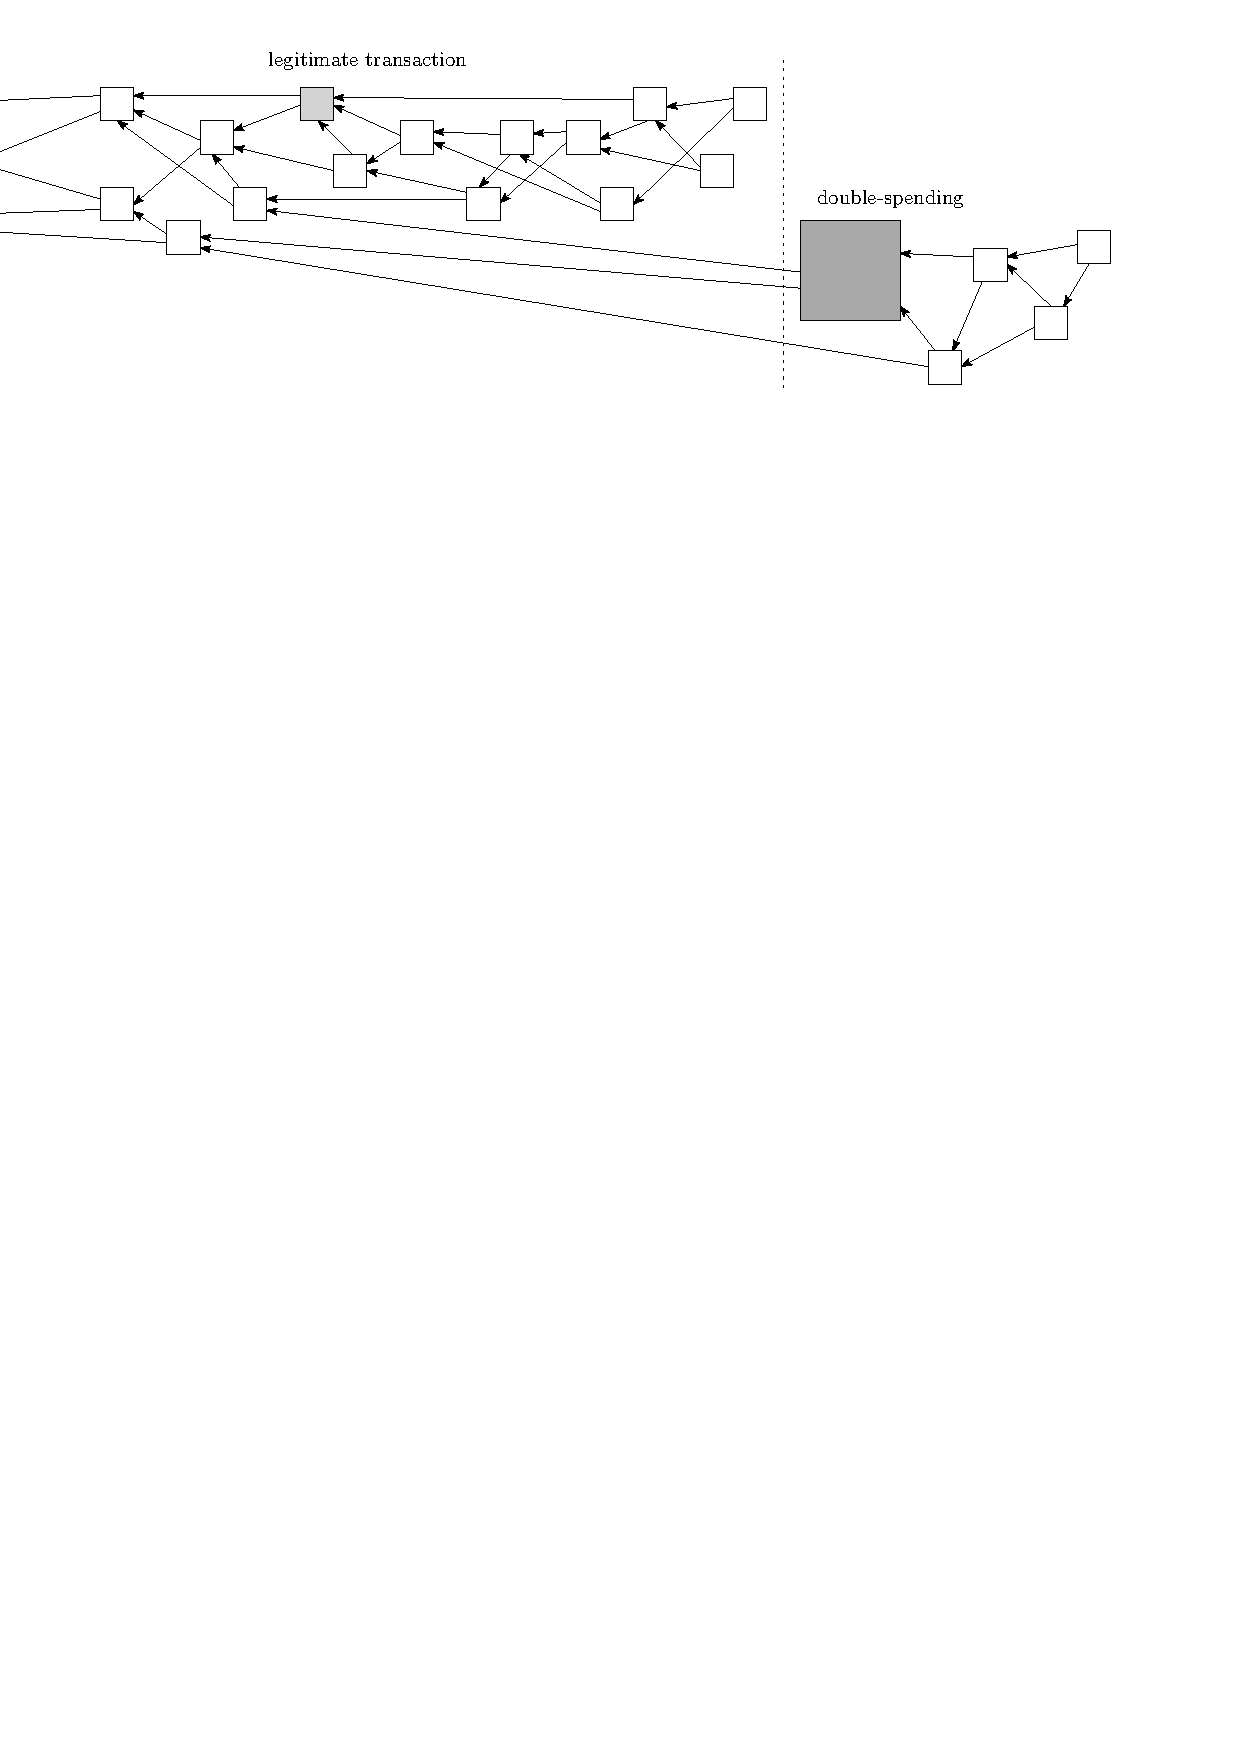
\includegraphics[width=\textwidth]{bigPoW} 
 \caption{「大權重」攻擊}
 \label{f_bigPoW}
 \end{figure}
這種成功攻擊的概率是
\[
 \IP[W^{(n_0)}<t_0]=1-\exp(-t_0\mu 3^{-n_0})
  \approx 1-\exp(-t_0\mu w_1^{-1})
  \approx \frac{t_0\mu}{w_1}.
\]
在 $\dfrac{t_0\mu}{w_1}$ 很小的情況下,這個近似是合理的假設。
然而,如果這種「即刻」攻擊沒有成功的話,攻擊者可以繼續尋找 nonce 以使得權重為 $3^n$ ,
其中 $n>n_0$,並希望在找到 nonce 的時候,合法交易分支的總權重要小於 $3^n$。這種情況的機率是
\[
 \IP[\lambda w W^{(n)}<3^n]
=1-\exp\big(-\mu 3^{-n_0}\times (3^{n_0}/\lambda w)\big)
  = 1-\exp(- \mu/\lambda w)
  \approx \frac{\mu}{\lambda w}.
\]

也就是說,儘管 $\dfrac{\mu}{\lambda w}$ 一般情況下應該是很小,在每一個 $n$ 值水準下,攻擊成功具有恒定的機率。
因此,最終總是可以攻擊成功。通常攻擊成功的須費時約 $3^{\lambda w/\mu}$ 。儘管這個數量可能非常大,
但是「第一次」\footnote{在時間 $t_0$ 內}成功攻擊的機率仍不容忽視。因此我們需要對策:
其一便是限制最大權重的值,甚至是設為固定常數值。如前面第~\ref{s_cutsets} 節所提到的,
後面的那種策略也許不是最好的方案,因為那樣不能為大量垃圾交易攻擊提供足夠的保護。


\medskip

那麼現在我們來討論當最大權重具有上限,且上限為 $1$ 時,估算攻擊成功的概率。 

假設給定的一筆交易在發送後經過 $t_0$ 個時間單位後,獲得累積權重為 $w_0$ ,
並假設這筆交易的調整階段已經結束,因此其累積權重以 $\lambda$ 的速度線性增長。
現在,想像攻擊者試圖對這筆交易進行雙重支付攻擊;為此,
他隱密的準備了雙重支付交易,並在商家決定接受第一筆合法的\emph{原始}交易之後開始生成\emph{其他的}交易來驗證這筆雙重支付交易
\footnote{或是在更早的時候; 稍後討論這個情況}。

若攻擊者的 subtangle 的權重要大於合法交易 subtangle 的權重的話,雙重支付攻擊就會成功。
如果在商家決定接受這筆合法交易後,攻擊者的 subtangle 在某個時刻超越了合法的 subtangle,則雙重支付的攻擊便會成功。
如果上述情況不出現的話,那麼雙重支付就不會被其他交易驗證,因為合法的交易獲得更多的累積權重並且最終所有新的 tips 都會間接驗證這筆交易,
因此雙重支付也就成為了孤立交易了。

如前所述,假定 $\mu$ 為攻擊者的計算能力,我們也假設交易是立即被傳播出去的。
假定 $G_1,G_2, G_3,\ldots$ 是以 $\mu$ 為參數\footnote{期望值為 $1/\mu$}的獨立同分佈的指數分佈變數,
並定義 $V_k=\mu G_k$,$k\geq1$。接著,$V_1, V_2,V_3...$ 是以 $1$ 為參數的獨立同分佈的指數分佈的變數。

假設在 $t_0$ 時刻商家決定接受交易其累積權重為 $w_0$ 。
讓我們來估算一下攻擊者成功完成雙重支付攻擊的機率。
記 $M(\theta)=(1-\theta)^{-1}$ 記作指數分佈參數為 $1$ 的動差生成母函數,
(參考文獻~\cite{Ross} 中~7.7 節)。對於 $\alpha\in(0,1)$\footnote{這是所謂的大偏差定理 (Large Deviation Principle) 的影響
參照書籍~\cite{DZ}, 以及~\cite{Ross} 第~8.5 節的定理~5.2 中簡單且有建設性的導出上限值。
還有~\cite{Dur} 第~1.9 對下限值的推導(較困難)。},
於是有如下公式成立:
\begin{equation}
\label{Chernoff}
 \IP\Big[\sum_{k=1}^n V_k \leq \alpha n\Big] \approx
   \exp\big(-n\phi(\alpha)\big), 
\end{equation}
其中 $\phi(\alpha)=-\ln \alpha + \alpha -1$ 是對 $\ln M(-\theta)$ 的拉格朗日轉換。
一般而言,當 $\alpha\in(0,1)$,$\varphi(\alpha)>0$ 是成立的。回顧指數隨機變數 Exp(1) 的期望值等於~$1$)。

假設 $\frac{\mu t_0}{w_0}<1$,否則,攻擊者的 Subtangle 最終超過合法的機率就接近於~$1$。
現在,為了在 $t_0$  時刻超過 $w_0$ ,攻擊者需要在 $t_0$ 時間單位內至少發送 $w_0$ 筆最大權重為 $m$ 的交易。
因此,通過公式~\eqref{Chernoff},我們可以得到雙重支付交易在 $t_0$ 時刻有更大累積權重的機率大概是
\begin{align}
 \IP\Big[\sum_{k=1}^{w_0/m} G_k  < t_0\Big]
 & = \IP\Big[\sum_{k=1}^{w_0} V_k  < \mu t_0\Big]
\nonumber\\
& = \IP\Big[\sum_{k=1}^{w_0} V_k  < w_0
\times\frac{\mu t_0}{w_0}\Big]
\nonumber\\
 & \approx \exp\big(-w_0
\phi\big(\textstyle\frac{\mu t_0}{w_0}\big)\big).
\label{double_t0}
\end{align}
也就是說,為了讓上面的機率非常小,我們需要 $\frac{w_0}{m}$ 很大,且 $\phi\big(\textstyle\frac{\mu t_0}{w_0}\big)$ 不能非常小。

注意到,在~$t\geq t_0$ 時刻時,合法交易的累積權重約為~$w_0+\lambda (t-t_0)$,因為我們假設適應階段已經結束了,
因此累積權重是以~$\lambda$ 的速度增加。
類似於~\eqref{double_t0},可以得到在~$t\geq t_0$ 時,雙重支付交易會有較大權重的機率約為:
\begin{equation}
\label{double_t}
 \exp\big(-(w_0+\lambda (t-t_0))
\phi\big(\textstyle\frac{\mu t}{w_0+\lambda (t-t_0)}\big)\big).
\end{equation}
接著,必須確保 $\frac{\mu t_0}{w_0}\geq 
\frac{\mu}{\lambda}$ , 因為在適應期間累積權重是以低於~$\lambda $ 的速度增加。
可以得到成功進行雙重支付的機率大概為:
\begin{equation}
\label{double_ever}
 \exp\big(-w_0\phi\big(\max(\textstyle\frac{\mu t_0}{w_0},
\frac{\mu}{\lambda})\big)\big).
\end{equation}
比如,假設 $\mu=2$, $\lambda=3$,因此攻擊者的計算能力只是比網路中其他所有的計算力稍微小一點點。
假設在時間~$12$ 的時候,交易的累積權重為~$32$。那麼,
$\max(\frac{\mu t_0}{w_0},\frac{\mu}{\lambda}) = \frac{3}{4}$,
$\phi\big(\frac{3}{4}\big)\approx 0.03768$,
且公式~\eqref{double_ever} 給出的上限大概是$0.29$。然而,若我們假設 $\mu=1$,並保持其他參數不變, 
那麼 $\max(\frac{\mu t_0}{w_0},\frac{\mu}{\lambda}) = \frac{3}{8}$,
$\phi\big(\frac{3}{8}\big)\approx 0.3558$,
而公式~\eqref{double_ever} 得到大約是 $0.00001135$,確實有很大的變化。

通過上述討論,我們觀察到很重要的一點就是,為了系統的安全,
必須確保 $\lambda > \mu$。也就是說,「誠實」節點的交易流量應該比攻擊者的計算能力大。
否則,公式~\eqref{double_ever} 的估算就沒有什麼用。
這也意味著需要額外的安全措施,例如在 tangle 基礎的系統發展的早期,設立檢查點。

對於如何決定兩個相互衝突的交易中哪一筆是合理的交易的策略來說, 
僅依靠累積權重判斷的我們必須十分小心謹慎。
這是因為可能是攻擊的目標,如同在~\ref{s_parasite} 節中所描述的攻擊。
攻擊者也許會事先准備好雙重支付交易,構建一個 subtangle 來指向驗證這筆雙重支付交易,
然後在商家接受合法交易之後將這個 subtangle 廣播出去。在下一節中我們將提出一個更好的方法來處理兩筆相互衝突的交易:
運行 tip 選擇演算法,然後看這兩筆交易中哪一筆交易被選取的 tip 所間接驗證。

\subsection{A parasite chain attack and a new tip 
selection algorithm}
\label{s_parasite}
Consider the following attack (Figure~\ref{f_tip_Markov}):
an attacker secretly builds a subtangle that occasionally 
references the main tangle to gain a higher score. 
Note that the score of honest tips is roughly the sum 
of all own weights in the main tangle, while the score
of the attacker's tips also contains the sum of all own weights in the
parasite chain.
Since network latency is not an issue for an attacker
 who builds a subtangle 
alone\footnote{This is due to the fact that an attacker can always
approve their own transactions without relying on any
information from the rest of the network.},
they might be able to give more height
to the parasite tips if they use a computer 
that is sufficiently strong. Moreover, the attacker can artificially 
increase their tip count at the moment of the attack by 
broadcasting many new transactions that approve 
transactions that they issued earlier on the parasite chain
%Finally, the number of attacker's tips 
%can be artificially increased at the moment of the attack
%(by issuing a lot of transactions that all approve
%\emph{the same} attacker's transactions,
%see 
(Figure~\ref{f_tip_Markov}).
This will give the attacker an advantage in the case where 
the honest nodes use some selection strategy 
that involves a simple choice between available tips.

To defend against this attack style,
we are going to use the fact that the main tangle is supposed
to have more active hashing power than the attacker. Therefore, the 
main tangle is able to produce larger increases in cumulative weight 
for more transactions than the attacker.  
%manages to give more cumulative weight to more transactions than the attacker.
The idea is to use a MCMC algorithm
to select the two tips to reference. 

Let $\HH_x$ be the current cumulative weight of a site.
 %(i.e., a transaction represented on the tangle graph). 
 Recall that we assumed all 
own weights are equal to~$1$. Therefore, the cumulative weight of a tip
is always~$1$, and the cumulative weight of other sites is at least~$2$.

The idea is to place some particles, a.k.a.\ random walkers,
on sites of the tangle and let them walk towards the tips
in a random\footnote{There is not a ``canonical'' source of randomness.
The nodes just use their own (pseudo)random number generators
to simulate the random walks.} way. The tips ``chosen'' by the walks
are then the candidates for approval.
The algorithm is described in the following way:
\begin{enumerate}
 \item Consider all sites on the interval $[W,2W]$, where 
 $W$ is reasonably large\footnote{The idea is to place the particle ``deep'' into
the tangle so that it will not arrive at a tip straight away. However, the 
particle should not be placed ``too deep'' because it needs to find a tip
 in a reasonable time. Also, the interval $[W,2W]$ is arbitrary. 
One could chose $[W,5W]$, etc.
There are also other ways to select the walkers' starting points.
 For example, a node can simply
take a random transaction received between $t_0$ and
$2t_0$ time units in the past, where~$t_0$ is some fixed time point.}.
% transactions with cumulative weight
% between $W$ and (say) $2W$ (where~$W$ 
%is reasonably large, to be chosen

 \item Independently place $N$ particles on sites in that
  interval\footnote{This choice
is largely arbitrary. We use several particles instead of just two
for additional security. The idea is that if a particle
were to accidentally jump to the attacker's chain, which is supposed
to be long, then it would spend a lot of time there 
and other tips will be chosen first.}.
  % there ($N$ is not so big, say, $10$ or so
 
 \item Let these particles perform independent
 discrete-time random
 walks ``towards the tips'', meaning that a transition
  from~$x$ to~$y$
is possible if and only if~$y$ approves~$x$
 \item The two random walkers that reach the tip set first will
sit on the two tips that will be approved.
However, it may be wise to modify this rule in the 
following way: first discard those random walkers that 
reached the tips \emph{too fast} because they may have ended on one
of the ``lazy tips''.
 \item The transition probabilities
 of the walkers are defined in the following
 way: if~$y$ approves~$x$ ($y\rightsquigarrow x$), 
then the transition probability~$P_{xy}$
 is proportional to $\exp\big(-\alpha(\HH_x-\HH_y)\big)$,
that is
 \begin{equation}
  \label{trans_probs}
   P_{xy} = \exp\big(-\alpha(\HH_x-\HH_y)\big)
\Big(\sum_{z: z \rightsquigarrow x}
 \exp\big(-\alpha(\HH_x-\HH_z)\big)\Big)^{-1},
 \end{equation}
where $\alpha>0$ is a parameter to be chosen\footnote{One can start 
with $\alpha=1$.}.
\end{enumerate}
Note that this algorithm is ``local'', meaning one does not need
 to traverse the tangle back to the genesis to perform relevant calculations.
In particular, 
observe that one does not need to calculate the cumulative
weights for the whole tangle. At most one needs to calculate the 
cumulative weights 
for the sites that indirectly approve the starting point
of the walker.


\begin{figure}
 \centering 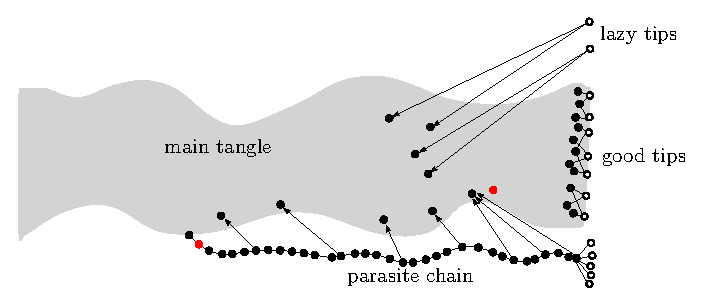
\includegraphics[width=0.81\textwidth]{tip_Markov} 
\caption{Visual representation of the tip selection algorithm for 
honest tips, as well as the parasite chain. The two red circles 
indicate an attempted double-spend by an attacker.
%On the tip selection algorithm. The two red circles indicate
%an attempted double-spend.
}
\label{f_tip_Markov}
\end{figure}

To check that the algorithm works as intended, first consider the ``lazy
tips''. These tips intentionally approve some old transactions
to avoid doing verification work (Figure~\ref{f_tip_Markov}).
Even if the particle 
is on a site approved by a lazy tip, it is not probable that the lazy
tip would be selected because the difference between cumulative
 weights would be very large and~$P_{xy}$ would be small.
 %, look at~\eqref{trans_probs}.

Next, consider this alternate attack style: the attacker secretly builds
a chain 
%(a ``parasite chain'')
 containing a transaction that empties their account balance to 
another account under their control, indicated as the leftmost red
circle in Figure~\ref{f_tip_Markov}. Then, the attacker
issues a transaction on the main tangle, represented by the rightmost red circle,
and waits for the merchant to accept it. The parasite chain occasionally
references the main tangle. However, the cumulative weight is not very 
large in the parasite chain. It should be noted that the parasite chain cannot 
reference the main tangle after the merchant's transaction. Furthermore, 
% and so its sites have
%good height/score (even better than those of the main tangle),
%although the cumulative weight is not so big in that chain. 
%Note also that it cannot reference the main tangle after 
%the merchant's transaction. Also, 
the attacker might try to artificially
inflate the number of tips in their parasite chain 
at the moment of the attack (Figure~\ref{f_tip_Markov}).
%as shown on the picture. 
The attacker's idea is to make the nodes issuing new transactions 
reference the parasite chain so that the honest branch of the tangle will
be orphaned.

It is easy to see why the MCMC selection algorithm
 will not select one of the attacker's tips with high probability.
%Basically, the 
The reasoning is identical to the lazy tip scenario:
%the same as why the algorithm does not 
%select the lazy tips:
 the sites on the parasite chain will
have a cumulative weight that is much smaller 
than the sites that they reference on the main tangle.
 Therefore, it is not probable that the random
walker will ever jump to the parasite chain unless it begins there,
and this event is not very probable either because the main tangle contains
more sites. 

As an additional protecting measure, we can 
first ran a random walk with a large~$\alpha$ (so that it is 
in fact ``almost deterministic'') to choose a 
 ``model tip''; then, use random walks with small~$\alpha$
for actual tip selection, but verify if the (indirectly)
referenced transactions are consistent with the model tip.

Observe also that,
for a random walk that \emph{always} moves towards the tips 
it is very simple and rapid to calculate the exit probability distribution using a straightforward recursion; this is something
that we \emph{do not} want the nodes to do. 
However, it is possible to modify our approach in the following
way: on each step, the random walk may
 backtrack (i.e., go 1 step away from the tips) 
with probability (say) $\frac{1}{3}$ 
(and divide the remaining $\frac{2}{3}$ as before). 
The walk will reach the tips very queckly anyway 
(because it has a drift towards the tips), 
but it will not be so easy to calculate the exit measure. 
% It is good that it's not easily calculable -- 
% the "selfish" nodes won't have easy time.

Let us comment on why 
 the nodes would follow this algorithm.
Recall from Section~\ref{s_general} that
it is reasonable to assume that at least a ``good'' proportion
of the nodes will follow the \emph{reference} algorithm.
Also, because of computational and network delays, the 
tip selection algorithm would rather work with a past snapshot
of the tangle with respect to the moment when a transaction
is issued. \emph{It may be a good idea to intentionally
move this snapshot to a time point further in the past\footnote{First
the random walker finds a former tip with respect to that snapshot,
and then it continues to walk towards the ``actual'' tips
on the current tangle.}} in the reference algorithm 
for the reasons that we explain in the sequel.
Imagine a ``selfish'' node that just wants to maximize 
the chances of their transaction being approved quickly.
The MCMC algorithm of this section, which is adopted by a
 considerable proportion of nodes, 
defines a probability
distribution on the set of tips. 
It is clear that a natural first choice for a selfish node would be
to choose the tips where the maximum of that distribution 
is attained. However, if many other nodes also behave
in a selfish way 
%(which is quite reasonable to assume as well)
 and use the same strategy, which is a reasonable assumption, 
 then they all 
will lose. \emph{Many} new transactions will approve 
the same two tips at roughly the same time, therefore
generating too much competition between them for subsequent approval.
It should also be clear that nodes will not immediately ``feel'' the cumulative 
weight increase caused by this mass approval of the same two tips since 
the nodes are using a past snapshot.
%Since the nodes use a past snapshot, they will not yet ``feel''
%the cumulative weight increase caused by this mass approval
%of the two tips.
 For this reason, even a selfish node would have 
to use some random tip approval algorithm\footnote{as noticed
before, for a backtracking walk there 
seem to be no easy way to discover which tips are 
 better (that is, more likely to be selected
by ``honest'' nodes) other than running the MCMC many times.
However, running MCRW many times requires time and other
resources; after one spends some time on it, 
the state of the tangle will already change, 
so one would possibly even have to start anew.
This explains why nodes do not have reasons
to abandon the MCMC tips selection strategy in favor
of something else, at least if they assume that a 
considerable proportion of the other nodes follow
the default tips selection strategy.}
 with a 
probability distribution for tip selection that is close to
% the selected tips should
%be, in some sense, ``not far away'' from
 the default probability distribution produced
by the reference tip selection algorithm.
We do not claim that this ``aggregated'' probability
distribution
would be equal to the default probability distribution in the presence of selfish nodes. 
However, the above argument shows that it should be close to it.
This means that the probability of many nodes attempting 
to verify the same ``bad'' tips would remain small. 
% selecting ``bad'' tips would remain small. 
In any case, 
%(differently from Bitcoin), 
there is not a large incentive for the nodes to be selfish 
because possible gains only amount to a slight decrease 
in confirmation time. This is inherently different from other 
decentralized constructs, such as Bitcoin. The important 
fact is that nodes do not have reasons to abandon the
 MCMC tip selection algorithm.


We would like to mention that the definition of transition 
probabilities, as given in~\eqref{trans_probs}, has not been 
set in stone.
% Also, it is not set in stone that the transition probabilities
%should necessarily be defined as in~\eqref{trans_probs}.
Instead of the exponent, one can use a different function 
that decreases rapidly, such~$f(s)=s^{-3}$. 
There is also freedom for choosing~$W$ and~$N$ as well.
At this point in time, it is unclear if there are any theoretical 
arguments that show exactly in which way these parameters 
should be chosen. In sum, we feel that the main contribution 
of this section is the idea of using MCMC for tip selection.
%In fact, the author's feeling is that the main contribution
%of this section is the very idea of using MCMC for tip selection;
%it is unclear if there is any ``theoretical''
%argument that shows exactly in which way these parameters
%must be chosen.

\subsection{Splitting attack}
\label{s_splitting}
Aviv Zohar suggested the following attack scheme against the 
proposed MCMC algorithm.
In the high-load regime, 
an attacker can try to split the tangle into two branches 
 and maintain the balance between them.
This would allow both branches to continue to grow.  
The attacker must place at least 
two conflicting transactions at the beginning of the split to prevent an honest node from effectively joining the branches 
by referencing them both simultaneously.
% Thereby split the power of the entire network. The network itself 
% work (because of the use of MCMC) almost equally to both sectors 
% and an attacker would only spend a little to balance. 
% In other words, weak inhibitor valid decision at will and splits 
% the computing power of the network to monitor contradictory versions. 
% It can also incorporate double spend parallel attacks.
Then, the attacker hopes that roughly half of the network would
contribute to each branch so that they 
would be able to ``compensate'' for random fluctuations,
even with a relatively small amount of personal computing power. 
If this technique works, the attacker would be able to spend the same
funds on the two branches.

To defend against such an attack, one needs to use a
``sharp-threshold'' rule 
%(like ``select the longest chain'' in Bitcoin) 
that makes it too hard to maintain the balance
between the two branches. An example of such a rule is 
selecting the longest chain on the Bitcoin network. Let us 
translate this concept to the tangle when it is undergoing a 
splitting attack. Assume that
the first branch has total weight 537, and the second branch 
has total weight 528. If an honest
node selects the first branch with probability very close to~$1/2$,
then the attacker would probably be able to maintain the
balance between the branches. However, if an honest
node selects the first branch with probability
much larger than $1/2$, then the attacker would probably
be unable to maintain the
balance. The inability to maintain balance between the two branches in 
the latter case is due to the fact that after an inevitable random fluctuation,
the network will quickly choose one of the branches and abandon the other. 
In order to make the MCMC algorithm behave this way,
one has to choose a very rapidly decaying function~$f$,
and initiate the random walk at a node with
 large depth so that it is highly probable
that the walk starts before the branch bifurcation.
In this case, the random walk would choose the ``heavier''
branch with high probability, even if the difference in
 cumulative weight between the competing branches is small. 

It is worth noting that the attacker's task is very 
difficult because of network synchronization
issues: they may not be aware of a large number 
of recently issued transactions\footnote{The ``real''
cumulative weights may be quite different from 
what they believe.}. Another effective 
method for defending against a 
splitting attack would be for a sufficiently
powerful entity to instantaneously publish a large number
 of transactions on one branch, thus rapidly changing the power balance
and making it difficult for the attacker to deal with this change. 
If the attacker manages to maintain
the split, the most recent transactions will only have around $50$\%
 confirmation confidence (Section~\ref{s_general}), and the branches 
will not grow. In this scenario, the ``honest'' nodes may decide to start 
selectively giving their approval to the transactions that occurred before 
the bifurcation, bypassing the opportunity to approve the conflicting 
transactions on the split branches.
%only the pre-split transactions then (and, in particular,
%not approve neither of the two conflicting transactions).

One may consider other versions of the 
tip selection algorithm. For example, if a node sees
 two big subtangles, 
then it chooses the one with a larger sum of own weights 
before performing the MCMC tip selection algorithm outlined above.
%and then does the tip selection only there using the 
%above MCMC algorithm. 

The following idea may be worth considering for future implementations. 
One could make the transition probabilities defined 
in~\eqref{trans_probs} depend 
on both $\HH_x-\HH_y$ and $\HH_x$ in such a 
way that the next step of the Markov chain is almost deterministic
when the walker is deep in the tangle, yet becomes more 
random when the walker is close to tips. This will help avoid entering the 
weaker branch while assuring sufficient randomness when choosing the 
two tips to approve.
% (so that there is enough randomness in the choice
%of the two transactions to approve). 



\paragraph{Conclusions:}
\begin{enumerate}
 \item We considered attack strategies for when an 
attacker tries to double-spend by ``outpacing'' the system.
 \item The ``large weight'' attack means that, in order to 
double-spend, the attacker tries to give a very large weight
to the double-spending transaction so that it would 
outweigh the legitimate subtangle. This strategy would be 
a menace to the network in the case where the allowed own weight is
unbounded. As a solution, we may limit the own weight
of a transaction from above, 
or set it to a constant value.
 \item In the situation where the maximal own weight
of a transaction is~$m$, the best attack strategy
is to generate transactions with own weight~$m$
that reference the double-spending transaction. 
When the input flow of ``honest''
transactions is large enough compared to the 
attacker's computational power, the probability
that the double-spending transaction
has a larger cumulative weight can be estimated
using the formula~\eqref{double_ever} (see also
examples below~\eqref{double_ever}).
 \item The attack method of building a ``parasite chain''
makes approval strategies based on height or score
obsolete since the attacker's sites will have higher values 
for these metrics when compared to the legitimate tangle. On the other hand,
the MCMC tip selection algorithm described in Section~\ref{s_parasite}
seems to provide protection against this kind of attack.
\item The MCMC tip selection algorithm also offers protection against 
the lazy nodes as a bonus.
%As a 
%bonus, it also offers protection against the ``lazy nodes'',
%i.e., those that just approve some old transactions to avoid 
%doing the calculations necessary for validating the tangle.
\end{enumerate}



\section{Resistance to quantum computations}
\label{s_quantum}
It is known that a sufficiently large
 quantum computer\footnote{Still a hypothetical construct as of today.}
  could be very efficient for handling problems
that rely on trial and error to find a solution. The process of finding a nonce
in order to generate a Bitcoin block is a good example 
of such a problem. As of today, one must 
check an average of $2^{68}$ nonces to find a suitable hash
that allows a new block to be generated. 
 It is known (see e.g.~\cite{BHT}) that a quantum computer would need 
$\Theta(\sqrt{N})$ operations to solve a problem that is analogous to 
the Bitcoin puzzle stated above. This same problem would need
~$\Theta(N)$ operations on a classical computer.
Therefore, a quantum computer would be 
around $\sqrt{2^{68}}=2^{34}\approx 17$ billion times
more efficient at mining the Bitcoin blockchain than a classical computer.
Also, it is worth noting that
 if a blockchain does not increase its difficulty in response 
to increased hashing power, there would be an 
increased rate of orphaned blocks.

For the same reason, a ``large weight'' attack would also be much more 
efficient on a quantum computer.
%described above would also be much more efficient on a quantum
%computer. 
However, capping the weight from above, as suggested
in Section~\ref{s_attacks}, would effectively prevent
a quantum computer attack as well. This is evident in iota because 
the number of nonces that one needs to check in order
to find a suitable hash for issuing a transaction is not 
unreasonably large. On average, it is around~$3^8$. 
The gain of efficiency for 
an ``ideal'' quantum computer would therefore
be of order $3^{4}=81$, which is already quite 
acceptable\footnote{Note that $\Theta(\sqrt{N})$
could easily mean $10\sqrt{N}$.}.
More importantly, the algorithm used in the iota implementation 
is structured such that the time to find a nonce is 
not much larger than the time needed for other tasks that 
are necessary to issue a transaction. The latter part is much
 more resistant against quantum computing, and therefore 
 gives the tangle much more protection against an adversary with a 
 quantum computer when compared to the (Bitcoin) blockchain.



\section*{Acknowledgements}
The author thanks  Bartosz Kusmierz, Cyril Gr\"unspan,
Olivia Saa, and
 Toru Kazama who pointed
out several errors in earlier drafts, and James Brogan
for his contributions towards making this paper more readable.



\begin{thebibliography}{9}
% \bibitem{iota_crypto}
% \textsc{Jinn Labs} (2015)  Iota whitepaper.
\bibitem{iota} Iota: a cryptocurrency for Internet-of-Things.
See \texttt{http://www.iotatoken.com/}, and
\texttt{https://bitcointalk.org/index.php?topic=1216479.0}

\bibitem{bitcoinj}  bitcoinj.  
Working with micropayment channels.\\
\texttt{https://bitcoinj.github.io/working-with-micropayments}

\bibitem{dag_generalized_blockchain}
\textsc{people on nxtforum.org}  (2014)
DAG, a generalized blockchain.
\texttt{https://nxtforum.org/proof-of-stake-algorithm/dag-a-generalized-blockchain/}  (registration at \texttt{nxtforum.org} required)

\bibitem{red_balloons}
\textsc{Moshe Babaioff, Shahar Dobzinski, Sigal Oren, Aviv Zohar} (2012)
On Bitcoin and red balloons.
\textit{Proc.\ 13th ACM Conf.\ Electronic Commerce}, 56--73. 


\bibitem{Dur} \textsc{Richard Durrett} (2004)
Probability -- Theory and Examples.
\textit{Duxbury advanced series.}


\bibitem{dagcoin} \textsc{Sergio Demian Lerner} (2015)
DagCoin: a cryptocurrency without blocks.
\texttt{https://bitslog.wordpress.com/2015/09/11/dagcoin/}

\bibitem{SZ} \textsc{Yonatan Sompolinsky, Aviv Zohar} (2013)
Accelerating Bitcoin's Transaction Processing.
Fast Money Grows on Trees, Not Chains.
\texttt{https://eprint.iacr.org/2013/881.pdf}

\bibitem{SZ_SPECTRE} 
 \textsc{Yonatan Sompolinsky, Yoad Lewenberg, Aviv Zohar} (2016)
SPECTRE:
Serialization of Proof-of-work Events: Confirming Transactions via
Recursive Elections.
%Yonatan Sompolinsky, Yoad Lewenberg, and Aviv Zohar
\texttt{https://eprint.iacr.org/2016/1159.pdf}

\bibitem{LSZ} \textsc{Yoad Lewenberg, Yonatan Sompolinsky, Aviv Zohar} 
(2015)
Inclusive Block Chain Protocols.\\
\texttt{http://www.cs.huji.ac.il/\textasciitilde{}avivz/pubs/15/inclusive\underline{\phantom{m}}btc.pdf}

\bibitem{lightning}
\textsc{Joseph Poon, Thaddeus Dryja} (2016)
The Bitcoin Lightning Network:
Scalable Off-Chain Instant Payments.\\
\texttt{https://lightning.network/lightning-network-paper.pdf}

\bibitem{Ross_m} \textsc{Sheldon M.\ Ross} (2012) 
\textit{Introduction to Probability Models.} 10th ed.

\bibitem{braids}
\textsc{David Vorick} (2015)
Getting rid of blocks.
\texttt{slides.com/davidvorick/braids}


\bibitem{DZ} 
\textsc{Amir Dembo, Ofer Zeitouni} (2010)
\textit{Large Deviations Techniques and Applications.}
Springer.

\bibitem{Ross} \textsc{Sheldon M. Ross} (2009) 
\textit{A First Course in Probability.} 8th ed.

\bibitem{BHT} \textsc{Gilles Brassard, Peter HØyer, Alain Tapp} (1998)
Quantum cryptanalysis of hash and claw-free functions.
\textit{Lecture Notes in Computer Science} \textbf{1380},
163--169.


\end{thebibliography}
\end{CJK}
\end{document}
